\documentclass[conference]{IEEEtran}
\usepackage{amsmath,amssymb}
\usepackage{graphicx}
\usepackage{booktabs}
\usepackage{multirow}
\usepackage{xcolor}
\usepackage{tikz}
\usepackage{tabularx}
\usetikzlibrary{shapes.geometric,arrows.meta,positioning,fit,backgrounds}
\usepackage[T1]{fontenc}
\usepackage{cite}
\usepackage{url}
\hyphenation{Micro-services}

\begin{document}

\title{ALMS: A Fully-Local, Low-Resource Pipeline for Migrating Python Monoliths\\ to Containerised FastAPI Microservices}

\maketitle

\begin{abstract}
Automated pipelines for migrating monolithic applications to microservices increasingly rely on large language models, but the pipelines that reach furthest down the migration path --- proposing service boundaries, generating code, and producing a deployable artifact --- do so by depending on hosted commercial LLMs, vendor-specific serverless targets, or GPU fine-tuning, excluding developers without cloud budgets or GPU access and organizations that cannot send source code to a third-party API. This paper presents ALMS, a pipeline that migrates a Python monolith to containerised FastAPI microservices entirely on a single commodity laptop. ALMS separates deterministic structure from language-model transformation: an AST-derived call graph, filtered of non-architectural edges and reduced by seed-fixed community detection, selects service boundaries without a model in the loop, while a local model (served by Ollama) is responsible only for code and test generation inside a compile-gated retry loop. The entire pipeline runs offline at zero API cost. In a case-study run on a 1,578-line Flask monolith, deterministic filtering reduces the dependency graph by 56.1\% of its nodes and 61.0\% of its edges before boundary selection runs. The reported case study evaluates ALMS with a 30B-parameter Mixture-of-Experts local model (\texttt{qwen3-coder:30b}, $\sim$3.3B active parameters per token) whose quantised weights exceed the host's physical RAM and are served through Ollama's CPU memory-mapped weight paging; the full decompose-generate-test pipeline completed in a single unattended run whose wall-clock exceeded ten hours. All four proposed services compiled cleanly and were carried through code and test generation, producing 1,120 generated test cases across 570 files; the resulting \texttt{docker-compose} stack and its Nginx API gateway were brought up successfully for three of the four services, while the fourth --- a non-domain orchestration service that community detection could not assign a clean bounded context --- failed to start. ALMS does not claim to match the decomposition quality of fine-tuned or trace-based prior work; its contribution is a reproducible, openly available artifact demonstrating that a disciplined deterministic/LLM split lets a single developer's own hardware carry a full decompose-generate-test-deploy migration through to a deployable, if imperfect, microservice stack, at zero API cost and without a GPU.
\end{abstract}

\begin{IEEEkeywords}
monolith-to-microservice migration, large language models, software modernization, reproducibility, FastAPI, retrieval-augmented generation, local inference
\end{IEEEkeywords}

\section{Introduction}

Migrating a monolithic application to a microservice architecture is one of the most disruptive undertakings a software team can perform. It requires identifying seams in a codebase that was never designed to be split, defining service boundaries, rewriting request handling and data access around those boundaries, and re-establishing confidence that the new system behaves like the old one. The research literature confirms what practitioners already know from experience: migration efforts are largely manual, span months, and depend heavily on the individual engineer's judgment of where the seams lie \cite{hassan2024,saucedo2025}. Boundary identification in particular is repeatedly singled out as the hardest sub-problem, and systematic surveys of the area find that the great majority of proposed approaches evaluate on a single system in a lab setting and stop before producing anything a team could actually deploy \cite{hassan2024,saucedo2025,abgaz2023}.

Large language models have recently been applied to this problem, and the results are promising: LLM-driven pipelines can propose service boundaries directly from source code \cite{sellami2025} and can carry a migration all the way to a deployable cloud artifact \cite{chen2026}. But the pipelines that reach furthest down the migration path also carry the steepest resource requirements. Contrastive-embedding approaches to boundary selection require fine-tuning a language model, which in practice means GPU time and a curated corpus of existing microservice repositories \cite{sellami2025}. Pipelines that generate and deploy code typically orchestrate hosted, commercial assistants --- Cursor, Claude Code, and comparably large closed models --- calling out to cloud APIs for every generation step \cite{chen2026}. Both design points quietly assume an evaluator with a GPU budget, a cloud billing account, or both, and a willingness to send proprietary source code to a third-party API. That assumption excludes a large and legitimate constituency: students and independent developers without GPU access, small teams without a cloud budget, and organizations whose source code cannot leave their own infrastructure for privacy or regulatory reasons \cite{huang2024}.

This paper presents \textbf{ALMS} (Agentic Legacy Modernization System), a pipeline that migrates a Python monolith to a set of containerised FastAPI microservices entirely on a single commodity laptop. ALMS combines deterministic static analysis --- an AST-derived call graph reduced by community detection --- with a local, open-weight language model served by Ollama, used only for the code- and test-generation steps that genuinely require it, inside a validation loop that never asks one model to check another's output. Every stage runs offline, at zero API cost, and the boundary-selection step is seed-fixed so that the same input codebase produces the same decomposition on every run. ALMS does not claim to match the decomposition quality of trace-based or fine-tuned methods \cite{sellami2025,kalia2021}, nor the deployability guarantees of pipelines built on large hosted models \cite{chen2026}; its contribution is access --- showing that a structurally disciplined pipeline can push a local model, even a much larger one than prior local-only baselines have attempted, through the entire migration on hardware a single developer already owns.

This paper makes the following contributions:
\begin{itemize}
\item \textbf{A deterministic/LLM split for local migration.} A pipeline architecture in which boundary selection, output validation, and inter-agent data contracts are handled deterministically, and a local model is responsible only for code generation and test generation inside a bounded, gated compile-retry loop.
\item \textbf{A fully local, zero-cost, offline implementation.} An end-to-end system --- analysis, boundary proposal, code generation, test generation, and containerised deployment --- that runs on a CPU-only, RAM-constrained laptop with no calls to a hosted model provider, evaluated here with a 30B-class Mixture-of-Experts model served through CPU weight paging.
\item \textbf{A reproducible artifact.} A one-command (\texttt{--demo}) pipeline run, a seed-fixed clustering step, and the generated pipeline artifacts (analyzer output, architect output, generated services, and generated tests) that reproduce every number and figure in this paper from the open-source repository.
\item \textbf{An honest, single-case feasibility evaluation.} A case-study run that reports not only what worked --- all four proposed services compiling, a working API gateway, three of four containers booting --- but what did not: one non-domain service that failed to start, a test-generation stage whose output is not gated by the same compile-retry discipline as code generation and is measurably less reliable as a result (58.2\% of generated test files parse), and cross-service duplication of endpoints that the current data-contract schema does not prevent.
\end{itemize}

The remainder of this paper is organised as follows. Section II surveys related work in monolith decomposition and LLM-driven migration and positions ALMS against it. Section III describes the ALMS architecture. Section IV details the implementation and configuration used in this study. Section V reports the case-study evaluation. Section VI discusses threats to validity. Section VII outlines future work, and Section VIII concludes.

\section{Background and Related Work}

\subsection{Monolith-to-Microservice Decomposition}

Systematic reviews of the migration literature classify decomposition approaches by the input they analyse --- static source structure, dynamic runtime traces, or a combination --- and by the technique applied to that input, typically some form of clustering \cite{hassan2024,saucedo2025,abgaz2023}. Three independent systematic reviews published within the last three years reach the same conclusion from different corpora: decomposition research is dominated by single-system, lab-only evaluations that stop at a class-to-service partition and rarely produce a running artifact \cite{hassan2024,saucedo2025,abgaz2023}. \textbf{Mono2Micro} \cite{kalia2021} is the representative practical tool in the runtime-trace family: it records execution traces labelled with business use cases, builds a class-similarity measure from direct and indirect call patterns across those traces, and applies hierarchical agglomerative clustering to produce an explainable class-to-service partition. It was evaluated on seven JEE applications against four baselines and, separately, with a survey of 21 industry practitioners, and remains the reference point for what a ``practical, effective'' decomposition tool looks like. Its cost is instrumentation: a user must exercise the application's use cases (or have functional tests do so) to obtain the traces the technique needs, and, being trace- and class-oriented, it targets Java applications exclusively --- the decomposition literature as a whole skews heavily toward Java, leaving Python monoliths comparatively under-served \cite{saucedo2025}. Static approaches avoid the instrumentation cost but have historically relied on hand-designed features --- module dependency graphs, call adjacency, bag-of-words similarity --- that are acknowledged even by their successors to be ``insufficient to create domain-relevant representations'' \cite{sellami2025}.

\subsection{LLM-Based Decomposition and Migration}

Language models have been used to improve on both ends of that trade-off. \textbf{MonoEmbed} \cite{sellami2025} replaces hand-designed features with language-model embeddings of source code, benchmarking eighteen pre-trained models and then improving the best of them with contrastive triplet fine-tuning before clustering with affinity propagation. On eight Java monoliths it achieves the best aggregate decomposition-quality score against six baselines including Mono2Micro --- but the fine-tuning step requires a curated corpus of existing microservice repositories and, even with parameter-efficient LoRA adaptation, GPU time that a single-laptop setting cannot assume. Like Mono2Micro, MonoEmbed stops at the class-to-service partition and does not generate code. \textbf{Mono2Sls} \cite{chen2026} is the closest prior work to ALMS in shape and the pipeline this paper positions itself against most directly. It pairs a lightweight static analysis --- an HTTP-entry-point and call-graph extraction comparable in spirit to ALMS's Analyzer --- with four sequential tool-using LLM agents (Architect, CodeDeveloper, SAMEngineer, ConsistencyValidator) that carry a Python or JavaScript monolith all the way to a deployed AWS SAM serverless application. Evaluated on six reverse-engineered benchmark applications, it reaches 100\% deployment success and out-performs both commercial coding assistants (Cursor, Claude Code) and a same-input LLM baseline on end-to-end correctness. Its ablation is the single most load-bearing result for ALMS's own design bet: removing the static-analysis-driven Architect and falling back to an unguided agent drops deployment success from six of six to three of six and end-to-end correctness by 23.4 percentage points on the comparable subset, leading the authors to conclude that ``pipeline design appears to matter more than the choice of backbone model'' \cite{chen2026}. That conclusion is what licenses ALMS's central wager: if a disciplined pipeline structure contributes more than a stronger backbone, a small or resource-constrained local model inside such a structure should be able to substitute for the hosted, commercial-scale models (Cursor's Sonnet 4.5, Claude Code's Sonnet 4.6, DeepSeek-V3.2) that Mono2Sls's agents actually run on. Mono2Sls's own stated threat to validity --- that hosted LLM inference is non-deterministic and its evaluation reports only pass@1, leaving run-to-run variance unmeasured \cite{chen2026} --- is a gap ALMS is designed to close for the boundary-selection step specifically, by replacing the LLM Architect with a seed-fixed deterministic clustering stage. More broadly, a systematic literature review of over 300 LLM4SE studies finds decomposition and migration to be one of many software-engineering tasks where LLM adoption has accelerated but reproducibility and deployment evaluation remain the exception rather than the rule \cite{hou2024}.

\subsection{LLMs for Test Migration}

A separate line of work applies LLMs to the test artifact of a migration rather than to boundary selection or code generation: Yeh et al.\ use large language models to migrate test cases from a monolith to its microservice targets once service boundaries are already known \cite{yeh2024}. This treats test migration as its own problem, assumed downstream of decomposition. ALMS's Test-Gen agent occupies related territory --- it generates a test suite for each newly produced service directly from the generated code and its legacy counterpart, and pairs this with a shadow-testing engine that replays identical inputs through the legacy and generated callables for exact-match comparison --- but treats test generation as one stage of a single continuous pipeline rather than a standalone step, and targets behavioural parity rather than translating existing test code. As the case study in Section V shows, folding test generation into the same pipeline without extending it the same compile-retry discipline given to code generation (Section III.E) is itself a source of measurable output quality loss, distinct from anything Yeh et al.\ report.

\subsection{Grounding Code Generation and Local Deployment}

Small and local models are more likely to have incomplete or dated knowledge of fast-moving framework idioms, which motivates grounding their output in retrieved documentation rather than relying on parametric knowledge alone. Zan et al.\ address exactly this gap for private, unseen libraries: an APIFinder retrieval module surfaces relevant API documentation for a natural-language requirement, and an APICoder model is then prompted with the retrieved APIs rather than asked to generate from memory, yielding substantial pass@k gains over generation with no retrieval \cite{zan2023}. ALMS applies the same retrieve-then-generate template to a knowledge base of FastAPI, DDD, security, and testing pattern documents, scoped per agent, to compensate for what a small local model does not reliably know about current framework conventions. Running that model locally rather than through a hosted API is itself motivated by a broader privacy and compliance argument: organizations that must keep source code in-house need to deploy language models on their own infrastructure \cite{huang2024}. Huang et al.\ study the harder version of that problem --- how to deploy a \textit{closed-source} model on-premises without exposing it to model-extraction attacks --- and propose selectively securing only the early transformer layers \cite{huang2024}. ALMS does not face that problem at all: because it builds on an \textit{open-weight} model, there is no proprietary model to protect, so it obtains the privacy and offline benefits of on-premises deployment without any of the confidentiality engineering \cite{huang2024} requires.

Community detection over a dependency graph is itself a well-studied problem outside the software-engineering literature. ALMS's Architect stage uses the Louvain method \cite{blondel2008}, a greedy modularity-optimisation algorithm originally developed for very large social and biological networks, via its widely used Python implementation \cite{aynaud2020}; graph-clustering-based decomposition of monolithic systems more generally --- assigning modules to services by optimising a coupling/cohesion objective over the module dependency graph rather than learning an embedding --- has also been explored directly in the microservice-migration literature \cite{filippone2023}. Static call-graph extraction for Python specifically is also available as a standalone visualization tool: \textbf{Pyan3} \cite{pyan2024} performs offline AST-based call-graph generation comparable in spirit to the first half of ALMS's Analyzer stage, but stops at producing a call graph for human inspection (typically rendered with Graphviz) rather than feeding it into community detection or any downstream boundary-selection or code-generation step.

\subsection{Positioning}

Table~\ref{tab:comparison} summarises these systems along the dimensions that matter for accessibility: boundary method, how far the pipeline reaches (decompose / generate / test / deploy), LLM hosting, hardware, API cost, offline capability, human-in-the-loop governance, and evaluation scale. Every prior automated pipeline either stops at the partition --- Mono2Micro \cite{kalia2021} and MonoEmbed \cite{sellami2025} both end at a class-to-service assignment --- or reaches a deployable artifact only by depending on hosted commercial LLMs and a vendor-specific serverless target, as Mono2Sls does \cite{chen2026}. None combines a full decompose-generate-test-deploy pipeline with a fully local, zero-cost, offline execution model. That is the gap ALMS occupies, at the explicit cost of the decomposition quality that fine-tuned or trace-based methods provide.

\section{Approach}

\subsection{Overview}

ALMS takes a directory of Python source files as input and produces a set of containerised FastAPI services, one generated test suite per service, and a \texttt{docker-compose.yml} that runs them together. The transformation is organised as a seven-stage pipeline (Fig.~\ref{fig:pipeline}): (1) deterministic structural analysis, (2) service-boundary identification, (3) a human review gate, (4) per-service code generation inside a compile--retry loop, (5) per-service test generation, (6) a second human review gate, and (7) artifact serialisation. Stages 1--2 use no language model; stages 4--5 use a single local model; a retrieval component supplies pattern guidance to every LLM stage.

The design is organised around one principle: \textbf{keep everything that can be made deterministic outside the language model, and give the model only the transformation step it is actually good at.} Boundary selection is a graph-clustering problem, so ALMS solves it with community detection rather than prompting. Output validation is a compiler problem, so ALMS gates every generated service with \texttt{py\_compile} and loops on failure. Inter-stage data contracts are schema-validation problems, so ALMS encodes them as typed records that are checked without a model in the loop --- an LLM is never asked to judge another LLM's output \cite{chen2026}. What remains for the model is: given a bounded set of source modules, a target framework, and retrieved idioms, emit the corresponding service. This division is what lets a local model stand in for the hosted commercial assistants used by comparable pipelines \cite{sellami2025,chen2026}; prior work reports that pipeline structure contributes more to migration quality than backbone-model strength \cite{chen2026}.

\subsection{Deterministic Structural Analysis}

The Analyzer parses every \texttt{.py} file with Python's \texttt{ast} module and extracts, per module: function definitions (name, parameters, called names, cyclomatic complexity, lines of code, docstring), class definitions (methods, base classes), \texttt{import} and \texttt{from...import} statements, and module-level assignments. Cyclomatic complexity is computed by counting decision points (\texttt{if}, \texttt{for}, \texttt{while}, \texttt{except}, boolean operators) rather than invoking an external metric tool, so the metric is reproducible across environments.

From this structure the Analyzer builds a directed dependency graph whose nodes are modules, functions, and classes. Edges are added only for relationships that correspond to real code entities: a call is linked to its resolved internal target if one exists, or to a third-party module if the call's head matches a known import; inheritance edges are added only to classes or imported modules actually observed. Calls that resolve to Python builtins, standard-library methods, or local-variable methods are \textbf{not} added as edges, because they are not architectural dependencies and would otherwise dominate both the coupling analysis and the subsequent clustering (Fig.~\ref{fig:graphfilter}). The graph is then reduced to a list of coupling hotspots (modules with cross-module fan-out above a threshold) and a set of circular dependencies (via strongly connected components). A SHA-256 hash over the sorted source contents is computed and used as a cache key, so re-running the pipeline on an unchanged codebase replays cached agent outputs instead of re-invoking the model.

The Analyzer's output is a typed \texttt{AnalyzerOutput} record --- codebase statistics, graph nodes and edges, hotspots, external dependencies, and cycles --- validated by schema, with no language model involved in its construction.

\subsection{Service Boundary Identification}

The Architect converts the directed dependency graph into an undirected weighted graph, using edge confidence as the weight, and applies the Louvain community detection algorithm \cite{blondel2008} (via \texttt{python-louvain} \cite{aynaud2020}) with a fixed random seed. Each resulting community becomes a candidate service. The service name is derived deterministically from the community's constituent modules, with a numeric suffix appended on collision so that distinct communities never produce colliding service identifiers. Each candidate is emitted as a \texttt{ServiceBoundary} record: name, bounded-context description, member modules, proposed endpoints, a confidence score, and a short rationale.

Optionally, the Architect prompts the model with the analysis summary and retrieved domain-driven-design guidance to refine or re-group the communities; when the model returns a well-formed set of boundaries these are used, otherwise the pipeline falls back to the raw community assignment. Because the fallback is deterministic and seed-fixed, the same input codebase yields the same decomposition on every run --- a property that hosted, non-deterministic pipelines cannot offer \cite{chen2026}. ALMS trades the decomposition quality of learned or trace-based methods \cite{sellami2025,kalia2021} for this determinism and for requiring neither training data, a GPU, nor runtime instrumentation. Section V.E shows a concrete case in which this fallback assigns a coherent bounded context to three of four communities but produces a fourth, low-confidence, non-domain ``catch-all'' service from the monolith's remaining orchestration glue code --- a known failure mode of community detection over hub modules that do not cleanly belong to any one domain, discussed further in Section VI.

\subsection{Retrieval-Augmented Generation}

Every LLM stage is grounded in a local knowledge base of short, curated migration-pattern documents. In the configuration evaluated in this study the knowledge base held 16 documents across five categories: FastAPI (5), refactoring (4), Docker/deployment (4), DDD (2), and security (1); documents are split into 500-character chunks with 100-character overlap, embedded with a local embedding model, and stored in a persistent on-disk vector index using cosine similarity. Each agent is bound to the subset of categories relevant to its task --- the Analyzer to refactoring patterns, the Architect to DDD patterns, the Refactoring agent to FastAPI and security (and, in the configuration used for the reported run, Docker) patterns, and the Test-Gen agent to a \texttt{testing\_patterns} category that the deployed knowledge base does not currently populate (Section VI) --- and retrieves up to a configured number of chunks per query, filtered by a 0.70 cosine-similarity threshold. The retriever returns chunks for prompt injection and performs no model synthesis of its own, mirroring the retriever-only design used elsewhere \cite{chen2026,zan2023}. Because the model is small relative to hosted alternatives and its training coverage of current framework idioms is limited, this retrieval step substitutes for knowledge the model does not reliably possess; embedding failures raise rather than silently returning a zero vector, so a degraded knowledge base cannot pass unnoticed.

\subsection{Code Generation and the Compile--Retry Loop}

For each proposed service the Refactoring agent receives the service's member modules with \textbf{full function bodies} (unlike the Analyzer, which sees only AST-level summaries), the target framework, and retrieved FastAPI and security patterns, and emits one or more Python files implementing the service as a FastAPI application with Pydantic schemas and SQLAlchemy models. Generated code is formatted with \texttt{black} and \texttt{isort} and then passed through a \texttt{py\_compile} gate. If compilation fails, the orchestrator loops back to the Refactoring agent with the error, for up to three attempts (configurable). If the service still does not compile after the last attempt, it is marked as needing human review and carried forward with that status rather than dropped. The retry loop is a genuine cycle in the execution graph (Fig.~\ref{fig:orchestrator}), and its firing rate is one of the properties measured in the Evaluation. This staged generate--check--regenerate structure is what allows a local model's first-attempt errors to be recovered automatically instead of surfacing as broken output \cite{chen2026}.

\subsection{Test Generation and Shadow Testing}

For each service that compiles, the Test-Gen agent generates a \texttt{pytest} suite --- happy-path, error-path, and property-based (\texttt{hypothesis} \cite{maciver2019}) cases --- from the generated service code and the corresponding legacy source. In addition, ALMS includes a shadow-testing engine that runs identical inputs through a legacy callable and its generated counterpart and compares outputs for exact match. This targets behavioural parity, the aspect of migration that decomposition-only approaches do not address \cite{sellami2025,kalia2021} and that a separate line of work tackles for the test artefact specifically \cite{yeh2024}. The shadow harness is currently exercised against in-process callables; wiring it to the running container stack is future work. \textbf{Unlike the Refactoring agent (Section III.E), Test-Gen output is not currently passed through a \texttt{py\_compile} gate or a retry loop} --- Fig.~\ref{fig:orchestrator} routes a compiled service directly to test generation with no cyclic recovery path. Section V.B reports the measurable consequence of that asymmetry.

\subsection{Orchestration: Fan-out, Reducers, and Human Gates}

The pipeline is a stateful graph. After boundary approval, the orchestrator issues one parallel branch per proposed service; each branch runs the compile--retry loop and then test generation as an isolated subgraph with its own attempt counter (Fig.~\ref{fig:orchestrator}). Branch results are merged back into a single list by a custom reducer keyed on service name, so that parallel branches never race and a re-run after a rejected final gate replaces a service's result rather than duplicating it.

Three human-in-the-loop gates punctuate the pipeline: after analysis, after boundary proposal, and after test generation. At each gate a reviewer may approve (continue), reject with feedback (re-run the preceding stage with that feedback), or stop (terminate). A command-line flag auto-approves every gate for unattended runs. These gates make the decomposition and the generated output auditable checkpoints rather than opaque end-to-end steps, which matters for the enterprise-migration setting that automated pipelines target \cite{kalia2021}.

\subsection{Output: Deployable Artifacts}

On completion the orchestrator writes, per service, the generated Python module(s), a \texttt{requirements.txt}, and a \texttt{Dockerfile}; a top-level \texttt{docker-compose.yml} wires the services on distinct ports behind an Nginx API gateway; and the generated test suites plus the analysis and architecture records are serialised as JSON. The result is a portable container stack that builds and runs with \texttt{docker compose}, with no dependency on a specific cloud provider --- in contrast to pipelines that target a single vendor's serverless platform \cite{chen2026} (Table~\ref{tab:comparison}).

\section{Implementation}

ALMS is implemented in Python across \texttt{core/}, \texttt{agents/}, \texttt{rag/}, \texttt{tools/}, \texttt{safety/}, \texttt{storage/}, and \texttt{ui/}. It has no cloud dependencies and is designed to run on a single commodity laptop; the reference configuration targets a 16~GB, CPU-only machine.

\subsection{Orchestration and models}

The pipeline graph is built with \textbf{LangGraph} \cite{langgraph2024}: a top-level \texttt{StateGraph} contains the analysis, boundary, and gate nodes, and a compiled subgraph for the per-service fan-out that contains the compile-retry cycle. LangGraph supplies the state machine, the cyclic compile-retry recovery loop, and the \texttt{Send} API used to dispatch the per-service fan-out in parallel; branch outputs are merged by a name-keyed reducer on the shared \texttt{service\_units} channel. The complete orchestration graph is implemented in \texttt{core/orchestrator.py}.

All model inference is local, served by \textbf{Ollama} \cite{ollama2024}. The configuration this study reports on uses \texttt{qwen3-coder:30b} for the Analyzer, Architect, Refactoring, and Test-Gen agents, and \texttt{nomic-embed-text} for embeddings. \texttt{qwen3-coder:30b} is a Mixture-of-Experts model: 30.5B total parameters, of which roughly 3.3B are active per token (8 of 128 experts fire per forward pass), quantised to Q4\_K\_M at approximately 19~GB on disk. Because that exceeds the 16~GB of physical RAM available on the reference machine, Ollama serves the model through llama.cpp's memory-mapped weight loading: pages of the GGUF file are pulled into RAM only as the corresponding layer or expert is touched, and cold pages are evicted under memory pressure. This makes a 30B-class model tractable on CPU-only, RAM-constrained hardware at the cost of latency --- every expert switch and context-window growth can trigger a fresh page fault from disk, and the reported case-study run's wall-clock exceeded ten hours as a result (Section V.A). The project's repository history also documents and validates a fully RAM-resident configuration using the smaller, fully-dense \texttt{qwen2.5-coder:7b} model (Table~\ref{tab:stack}), which fits in RAM without paging and completes individual pipeline runs an order of magnitude faster; this study reports on the larger, higher-quality, paging configuration because it is the one for which the artifact discussed in Section V was generated. Sampling temperature is low for analysis (0.05) and slightly higher for code (0.2) and test (0.15) generation.

\subsection{Data contracts}

Every inter-stage message is a Pydantic v2 model, validated on construction: \texttt{AnalyzerOutput} (statistics, graph nodes/edges, hotspots with confidence scores), \texttt{ArchitectOutput} (a list of \texttt{ServiceBoundary} records), \texttt{RefactoringOutput} (generated files plus \texttt{py\_compile} pass flag), \texttt{TestGenOutput} (test cases, shadow-test results, coverage target), and the per-branch \texttt{ServiceUnit} that carries a service through the fan-out with its compile-attempt count and review status. The orchestrator's own \texttt{PipelineState} records the project id, loaded source, current phase, all agent outputs, the human-approval history, an iteration counter, and an error list. Because these contracts are enforced by schema, a malformed agent response is caught at the boundary rather than propagating downstream, and no model is used to validate another model's output.

\subsection{Retrieval and storage}

The knowledge base is a set of Markdown pattern documents (Section III.D). It is chunked, embedded via Ollama, and stored in a persistent ChromaDB collection using cosine similarity; retrieval is filtered by a 0.70 minimum-similarity threshold and scoped per agent. Agent inference outputs are cached in a local disk cache keyed on the codebase hash, so unchanged inputs do not re-invoke the model. A SQLite audit database is designed to record every agent action (phase, duration, success, error, structured detail), every human decision (checkpoint, approval, feedback, iteration), and per-run metadata; in the reported case study this database was not retained alongside the generated artifact, so per-stage timing and peak-RAM figures below are reported only at the granularity the retained artifact supports (Section V.A, Section VI).

\subsection{Artifact and reproducibility}

The system is invoked from a single command-line entry point: \texttt{--init-kb} builds the knowledge base, \texttt{--demo} runs the pipeline on a bundled sample monolith, \texttt{--skip-hitl} runs unattended, and \texttt{--check} verifies the local environment. Generated output, the vector index, the cache, and the audit database are all regenerable and excluded from version control. Reproducibility rests on three choices: a fixed Louvain seed makes boundary selection deterministic; the codebase hash makes cached runs replay exactly; and local open-weight models remove dependence on a hosted endpoint whose behaviour can drift between runs. The residual source of run-to-run variance is the language model's own non-determinism at non-zero temperature, discussed in the Evaluation.

\subsection{Availability}

The implementation, the sample monolith, the knowledge base, and the generated case-study artifacts discussed in Section V are available in the project repository under its stated licence. This manuscript is being prepared for submission consideration to venues appropriate to a reproducible-systems and software-engineering-tools contribution, including \emph{PeerJ Computer Science}, \emph{SoftwareX}, \emph{Information and Software Technology}, \emph{Applied Sciences} (MDPI), and the \emph{Journal of Systems and Software}; final formatting will follow the target venue's requirements.

\begin{table*}[t]
\centering
\caption{ALMS Technology Stack (\texttt{config.yaml}).}
\label{tab:stack}
\begin{tabular}{ll}
\toprule
\textbf{Concern} & \textbf{Choice} \\
\midrule
Orchestration & LangGraph $\geq$0.1.0 \cite{langgraph2024} (\texttt{StateGraph}, \texttt{Send} fan-out, subgraph cycles), on LangChain Core \\
LLM runtime & Ollama \cite{ollama2024}, local; \texttt{qwen3-coder:30b} (MoE, 30.5B total / $\sim$3.3B active/token, Q4\_K\_M) --- reported case study; \\
 & \texttt{qwen2.5-coder:7b} (fully dense) also validated as a fully RAM-resident, lower-latency configuration \\
Embeddings & \texttt{nomic-embed-text} (via Ollama), 768-dim \\
Vector DB & ChromaDB (local, SQLite-backed), cosine similarity \\
Static analysis & \texttt{ast}, \texttt{networkx}, \texttt{python-louvain} \cite{aynaud2020} (Louvain method \cite{blondel2008}) \\
Schemas & Pydantic v2 (agent I/O contracts) \\
Codegen post-proc. & Jinja2, \texttt{black}, \texttt{isort}, \texttt{py\_compile} \\
Security & Bandit (optional) \\
Generated tests & \texttt{pytest}, \texttt{hypothesis} \cite{maciver2019} \\
Target services & FastAPI + SQLAlchemy + Pydantic, Docker / \texttt{docker compose} \\
Cache / audit & DiskCache, SQLite \\
UI & \texttt{rich} \\
\bottomrule
\end{tabular}
\end{table*}

\section{Evaluation}

ALMS is evaluated as a feasibility study, not a benchmark. The system is exercised end to end on a single input, \texttt{examples/sample\_monolith}: a 6-file, 1,578-line Flask application (76 functions, 7 classes, mean cyclomatic complexity 2.32) spread across six modules --- \texttt{app}, \texttt{database}, \texttt{models}, \texttt{orders}, \texttt{payments}, and \texttt{users}. This section reports what happened when the full pipeline ran on that input, organised around four research questions. Consistent with the framing of this paper as a system-and-artifact report, no claim is made that the results generalise beyond this one codebase; Section VI treats that limitation explicitly.

\subsection{RQ1: Does the pipeline complete on commodity, CPU-only hardware?}

The pipeline was run with \texttt{python main.py} on a CPU-only, 16~GB-RAM laptop, with all inference served locally by Ollama (\texttt{qwen3-coder:30b} for generation, \texttt{nomic-embed-text} for embeddings) and no GPU involved. The pipeline reached its terminal (\texttt{complete}) phase in a single unattended run whose total wall-clock exceeded ten hours --- consistent with the CPU-only memory-mapped paging behaviour described in Section IV.A, since the model's $\sim$19~GB of quantised weights do not fit in the host's 16~GB of physical RAM. Because Ollama serves the model locally and DiskCache replays agent outputs for an unchanged codebase hash, no run of this pipeline made a network call or incurred an API charge. Per-stage timing and peak-RAM figures were not retained alongside the generated artifact for this run (Section IV.C); we report this as a limitation in Section VI rather than presenting invented numbers. A companion run of the fully RAM-resident \texttt{qwen2.5-coder:7b} configuration (Table~\ref{tab:stack}) completed the equivalent pipeline in substantially less wall-clock time on the same hardware, at the cost of the lower generation quality reflected in that run's smaller three-service output; a controlled, timed comparison between the two configurations is future work (Section VII).

\subsection{RQ2: Is the generated output syntactically valid and bootable?}

\textbf{Code generation.} The Architect proposed 4 service boundaries; all 4 were carried through code generation, and all 4 of the generated service modules pass \texttt{py\_compile} with no service requiring the fallback ``needs human review'' status --- consistent with the compile-retry loop design of Section III.E.

\textbf{Test generation.} The Test-Gen agent produced 570 test files (1,120 test cases by the pipeline's own count) across the four services. Because Test-Gen output is not passed through a compile gate (Section III.F), we checked this directly: only 332 of the 570 generated test files (58.2\%) are importable, syntactically valid Python. The remaining 238 files (41.8\%) share a single, consistent failure mode --- an unterminated \texttt{from app import (} statement partway through the file's fixture header, together with decorator-only fixture stubs (e.g.\ \texttt{@pytest.fixture(autouse=True)} with no following function body) --- consistent with output truncation against the Test-Gen agent's context window rather than a logic error. This is a direct, measurable consequence of the asymmetry noted in Section III.F: the same discipline that gives code generation a 100\% \texttt{py\_compile} pass rate is not currently applied to test generation.

\textbf{Container deployment.} A full \texttt{docker compose up} of the generated stack, including the Nginx API gateway, was exercised against all four services. Three of the four containers --- User Management Service, Order Processing Service, and Payment Processing Service --- built and started successfully behind a working gateway. The fourth, Application Core Service, did not start. Application Core Service is notable in the Architect's own output: it is the lowest-confidence proposal (0.78 against 0.87--0.92 for the other three), owns no database tables, and is described by the Architect itself as a service that ``acts as an API gateway and orchestrator, coordinating calls between other services'' --- i.e.\ it is the monolith's residual request-handling glue code (\texttt{app.py}'s routes, request parsing, and response formatting) that the clustering step could not assign a clean bounded context, rather than a genuine domain service. We return to this in Section VI. We additionally observed that the Order Processing and Payment Processing services independently regenerate CRUD endpoints and models for \texttt{/users} and \texttt{/products} that are also, correctly, owned by User Management Service --- a data-ownership leak that the current schema contracts (Section IV.B) do not detect or prevent, discussed further in Section VI.

\subsection{RQ3: What effect does deterministic structural filtering have?}

Unlike RQ1/RQ2, this result requires no LLM and is fully reproducible from the static analysis alone: we compare the dependency graph the Analyzer would build without the builtin/stdlib/local-variable call filter described in Section III.B against the graph it actually builds, both computed directly from the current implementation against \texttt{sample\_monolith}. The unfiltered graph has 171 nodes and 267 edges and yields 6 coupling ``hotspots''; the filtered graph used by ALMS has 75 nodes and 104 edges and yields 2 hotspots --- a 56.1\% reduction in nodes and a 61.0\% reduction in edges (Fig.~\ref{fig:graphfilter}). The two hotspots that survive filtering are \texttt{app}, which fans out to \texttt{database}, \texttt{orders}, \texttt{payments}, and \texttt{users}, and \texttt{orders}, which fans out to \texttt{database}, \texttt{models}, \texttt{payments}, and \texttt{users} --- the two genuine god-modules in this monolith, as opposed to the mixture of god-modules and spurious builtin/stdlib ``coupling'' (\texttt{str}, \texttt{logger.info}, \texttt{datetime.now}, and similar) that the unfiltered graph reports. This matters beyond hotspot reporting: the same filtered graph, once built, is the input to Louvain community detection (Section III.C). An unfiltered graph in which every function is nominally coupled to \texttt{len}, \texttt{round}, and \texttt{ValueError} pollutes the clustering with edges that carry no architectural meaning --- precisely the condition under which a local model would otherwise have to reason about boundaries for a large codebase, not only a small one.

\subsection{RQ4: What is the resource and cost profile relative to a hosted pipeline?}

ALMS is not compared against Mono2Sls \cite{chen2026} on decomposition or correctness --- the two systems target different output platforms (portable containers versus AWS SAM) and were not run on the same benchmark. The comparison that is meaningful, Table~\ref{tab:comparison} reports, is qualitative: Mono2Sls's agents run on hosted, commercial-scale backbones (Cursor's Sonnet~4.5, Claude Code's Sonnet~4.6, DeepSeek-V3.2) and its own reported per-agent latency is 58--106 minutes dominated by paid cloud inference \cite{chen2026}; ALMS's entire run, including analysis, boundary selection, generation, and testing, costs \$0 in API fees and never leaves the host machine, at the explicit cost of the multi-hour wall-clock documented in RQ1 for a model large enough to be paged from disk. The trade-off is explicit and one-directional in this paper's framing: ALMS does not claim to match Mono2Sls's deployment success or its end-to-end correctness benchmark; it claims to reach a smaller but non-trivial point in the same design space (Sections III, VI) without a cloud dependency, a GPU, or a per-run bill.

\begin{table}[t]
\centering
\caption{Resource and Cost Profile (\texttt{sample\_monolith}, CPU-only).}
\label{tab:resources}
\begin{tabular}{@{}p{2.3cm}p{5.6cm}@{}}
\toprule
\textbf{Item} & \textbf{Value} \\
\midrule
Host & CPU-only laptop, 16~GB RAM, no GPU \\
Model (reported run) & \texttt{qwen3-coder:30b} (MoE, $\sim$3.3B active/tok) \\
Model weights on disk & $\sim$19~GB (Q4\_K\_M), exceeds host RAM \\
Serving strategy & Ollama, CPU mmap weight paging \\
Embedding model & \texttt{nomic-embed-text} \\
Total wall-clock & $>$10~h (single unattended run) \\
Per-stage timing & Not instrumented for this run (Sec.~VI) \\
Peak RAM & Not instrumented for this run (Sec.~VI) \\
API cost & \$0 \\
Network & Offline throughout \\
\bottomrule
\end{tabular}
\end{table}

\subsection{Case-study walkthrough}

Given \texttt{sample\_monolith}'s six modules, the Analyzer's filtered dependency graph (RQ3) is passed to the Architect, which runs Louvain community detection with a fixed seed. In the reported run the LLM-refinement step returned a well-formed boundary set for three of the four proposed services --- \textbf{User Management Service} (\texttt{users}, tables \texttt{users}, \texttt{user\_profiles}, \texttt{sessions}, \texttt{roles}; confidence 0.92), \textbf{Order Processing Service} (\texttt{orders}, tables \texttt{orders}, \texttt{order\_items}, \texttt{products}, \texttt{order\_status\_transitions}; confidence 0.89), and \textbf{Payment Processing Service} (\texttt{payments}, tables \texttt{payments}, \texttt{refunds}, \texttt{payment\_gateways}, \texttt{payment\_transactions}; confidence 0.87) --- plus the lower-confidence \textbf{Application Core Service} discussed in Section V.B (confidence 0.78, no owned tables).

For User Management Service, the Refactoring agent produced a 359-line FastAPI module exposing 13 endpoints, including:
{\footnotesize
\begin{verbatim}
@app.post("/users",
          response_model=User)
async def create_user(
    user: UserCreate,
    db: Session = Depends(get_db)
):
  existing = db.query(UserORM)\
    .filter(UserORM.email ==
            user.email).first()
  if existing:
    raise HTTPException(
      status_code=400,
      detail=f"User with email "
             f"{user.email} exists")
  hashed = hash_password(
             user.password)
  db_user = UserORM(
    email=user.email,
    name=user.name,
    hashed_password=hashed,
    role=user.role,
    is_active=user.is_active)
  db.add(db_user)
  db.commit()
  db.refresh(db_user)
  ...
  return db_user
\end{verbatim}
}
against a Pydantic \texttt{UserCreate} schema with a field validator enforcing a minimum password length, and a SQLAlchemy \texttt{UserORM} model with a uniqueness constraint on email --- a direct, compiling translation of the legacy \texttt{users.create\_user} function's validation logic into FastAPI's dependency-injected, schema-validated idiom. The corresponding \texttt{tests/User Management Service\_test\_create\_user.py} file --- one of the 332 syntactically valid test files (Section V.B) --- exercises this endpoint against a test client and asserts on the response body's email, name, role, default-active flag, and generated \texttt{id}/\texttt{created\_at} fields. The complete stack is wired by the generated \texttt{docker-compose.yml}, exposing each service on a distinct port behind the Nginx gateway on port 8080, which is the artifact this case study evaluates for build and boot validity in RQ2.

\section{Discussion and Threats to Validity}

\subsection{Discussion}

The results in Section V support a narrower claim than ``ALMS decomposes and migrates monoliths well'': they support ``the deterministic/LLM split described in Section III lets a local model --- including one much larger than prior local-only baselines have attempted --- reach a mostly-bootable, containerised output, at zero API cost, for at least one monolith.'' The RQ3 result is the clearest evidence for the design's internal logic --- removing spurious builtin- and stdlib-derived edges before clustering is what keeps the boundary-selection graph small and architecturally meaningful enough for community detection to operate on at all, independent of which model, if any, later refines the result. The RQ1/RQ2 results say the split is \textit{sufficient} to reach a bootable stack end to end for three of four proposed services on one small, low-complexity Flask application; they do not say the split is sufficient in general, and this paper does not claim that it does.

The Application Core Service failure is instructive rather than merely disappointing. Community detection assigns every module to some community; when a module's role in the codebase is orchestration and request routing rather than domain ownership --- as \texttt{app.py} is in this monolith --- Louvain has no mechanism to recognise that and will still emit a community for it, which the Architect then dresses with a plausible-sounding bounded-context description (``acts as an API gateway and orchestrator''). The resulting service has no data to own, no clear single responsibility, and, empirically, does not run. A pipeline that wants to handle this case would need either a pre-clustering heuristic that flags orchestration-only hub modules for different treatment, or a post-clustering check that a proposed service without owned tables is treated as high-risk and routed to mandatory human review rather than auto-approved. Neither exists in the current implementation.

The test-generation compile-validity gap (58.2\% of files, Section V.B) is a second instance of the same underlying lesson the rest of this paper argues for: the stages of ALMS that are protected by a deterministic gate (code generation, via \texttt{py\_compile} and retry) are reliable, and the one LLM-facing stage that is not similarly gated (test generation) is measurably less so. This is not evidence against the paper's central design principle; it is evidence \textit{for} it, in a place the current implementation has not yet applied it.

\subsection{Threats to Validity}

\textbf{Construct validity.} This study's success criteria --- the pipeline reaches its terminal phase, generated service files pass \texttt{py\_compile}, and the resulting containers build --- measure structural and syntactic validity, not behavioural correctness. The shadow-testing engine that compares legacy and generated outputs on identical inputs exists in the codebase but is currently exercised against in-process callables rather than the running container stack, so no result in this paper should be read as evidence of functional parity with the original monolith. Test generation is measured by file count and compile-validity, not by fault-detection ability or coverage.

\textbf{Internal validity.} The Louvain-based fallback used when the LLM does not return a well-formed boundary set tends to pull hub modules --- \texttt{app} in this monolith --- into a community of its own without owned tables or a clear domain, as Section VI.A discusses; the reported case study's \texttt{inter\_service\_calls} and \texttt{data\_ownership} fields, while populated for the three domain services, list only synchronous/asynchronous call directions rather than concrete contracts, and the Refactoring agent's independent, out-of-order regeneration of \texttt{/users} and \texttt{/products} CRUD logic inside Order Processing and Payment Processing Service (Section V.B) shows that data ownership as declared by the Architect is not currently enforced when those modules are later generated. Generation quality also depends on language-model sampling: temperature is greater than zero at every LLM stage, and the Ollama backend is not seeded, so repeated runs on the same input are not guaranteed to produce identical code, even though the boundary-selection step is. This paper reports a single run; run-to-run variance in compile-retry firings, needs-review counts, and generated-code content is uncharacterised. The audit database designed to record per-stage timing (Section IV.C) was not retained alongside the artifact analysed here, so the resource figures in Table~\ref{tab:resources} are reported only at the coarse, single-number granularity the retained artifact supports; a separate, earlier run of this pipeline on the same input under a smaller (7B) model configuration is known to have completed with a different, smaller decomposition (three services, 23 generated tests) and its own analyzer output reporting a graph with 134 nodes and 263 edges rather than the 75/104 recomputed directly from the current filtering implementation in RQ3 --- consistent with intervening fixes to the dependency-graph construction logic recorded in the project's own commit history between the two runs, and a reminder that ``the same codebase yields the same decomposition'' (Section III.C) is a property of a fixed version of the pipeline, not of the pipeline across its own development history.

\textbf{External validity.} The evaluation is a single case study on one 1.6-kLOC Flask monolith. No claim in this paper should be read as evidence about performance on larger codebases, other Python web frameworks, non-web applications, or languages other than Python --- all of ALMS's design assumptions (AST-based extraction, the \texttt{app.route}-oriented pattern library, the boundary-naming heuristic) are Python- and Flask-shaped. The single-model choice (\texttt{qwen3-coder:30b}) means the reported feasibility result is also specific to that model's capability and its CPU-paging latency profile; whether a smaller or differently-quantised local model reaches a similar decomposition and boot-success outcome in comparable wall-clock time is untested here beyond the single informal comparison against the \texttt{qwen2.5-coder:7b} configuration noted in Section V.A. Consistent with Section I, this paper frames these as an experience report's honest N=1 limitation rather than a benchmark claim, and Section VII outlines the multi-project and ablation work needed to narrow it.

\section{Future Work}

The most direct extension of this work is scale: running ALMS unattended over a corpus of 10--30 small and medium Python monoliths would replace the single case study in Section V with per-repository and aggregate statistics, and would let ablations of the design --- no retrieval, no compile-retry loop, no deterministic clustering, no human-in-the-loop gates --- be measured rather than argued for. Closing the behavioural-fidelity gap identified in Section VI requires wiring the existing shadow-testing engine to a live \texttt{docker compose up} deployment and replaying recorded monolith traffic against it, rather than comparing in-process callables. On the decomposition side, deriving \texttt{tables} and \texttt{inter\_service\_calls} from the static analysis --- rather than leaving them populated only when the model chooses to --- and allowing a reviewer to interactively nudge Louvain's community assignment at the human-in-the-loop gate would address the hub-module over-merging problem directly rather than only reporting it (Section VI.A); the same mechanism could flag a proposed service with no owned tables for mandatory review instead of auto-approval. Extending the same \texttt{py\_compile}-gated, bounded-retry discipline that Section III.E gives code generation to the Test-Gen agent's output (Section V.B, Section VI.A) is a small, concrete, and directly motivated next step, as is enforcing the data-ownership boundaries the Architect already declares so that sibling services stop regenerating one another's CRUD surface. Populating the currently empty \texttt{testing\_patterns} knowledge-base category (Section III.D) and instrumenting per-stage timing and peak-RAM consistently across runs (Section VI.B) would close two further gaps this study's Table~\ref{tab:resources} reports as absent rather than measured. Finally, a controlled, timed comparison of the fully RAM-resident \texttt{qwen2.5-coder:7b} configuration against the paged \texttt{qwen3-coder:30b} configuration reported here --- decomposition quality, compile/boot success rate, and wall-clock, on the same input --- would turn Section V.A's informal observation into a quantified result. The AST-based front end is Python-specific by construction; supporting additional languages would require a parallel structural analyzer per language, sharing the downstream boundary-selection, generation, and validation stages.

\section{Conclusion}

This paper presented ALMS, a pipeline that migrates a Python monolith to containerised FastAPI microservices entirely on a single commodity laptop, using a local language model, at zero API cost, offline, and reproducibly. Its central design decision is a strict separation of concerns: boundary selection, output validation, and inter-agent communication are handled deterministically --- by a filtered call graph, a seed-fixed community-detection algorithm, a \texttt{py\_compile} gate with bounded regeneration, and schema-checked data contracts --- so that the language model is responsible only for the code- and test-generation steps it is actually suited to. The case-study evaluation in Section V shows this split is sufficient to carry one representative monolith through the full pipeline to a mostly-bootable container stack --- three of four services running behind a working API gateway --- using a 30B-class Mixture-of-Experts local model an order of magnitude larger than prior local-only feasibility work has reported, and quantifies the effect of deterministic structural filtering directly: a 56.1\% reduction in graph nodes and a 61.0\% reduction in edges before boundary selection ever runs. It also reports, with the same directness, what did not work: one non-domain service that community detection could not cleanly assign a bounded context to, a test-generation stage whose output validity (58.2\%) lags the code-generation stage's (100\%) precisely because it lacks the same compile-retry gate, and cross-service data-ownership leakage the current schema contracts do not catch. ALMS does not match, and does not claim to match, the decomposition quality of fine-tuned or trace-based prior work, or the deployment scale of pipelines built on hosted commercial models. Its contribution is access: evidence that the full migration pipeline, including a substantially larger local model than prior local-only baselines have attempted, can run on hardware a single developer already owns, with an honest account of where that pipeline currently falls short.

\begin{thebibliography}{99}

\bibitem{hassan2024} H. Hassan, M. A. Abdel-Fattah, and W. Mohamed, ``Migrating from monolithic to microservice architectures: A systematic literature review,'' \textit{International Journal of Advanced Computer Science and Applications}, vol. 15, no. 10, pp. 104--116, Oct. 2024.

\bibitem{saucedo2025} A. Mart\'{i}nez Saucedo, G. Rodr\'{i}guez, F. Gomes Rocha, and R. Pereira dos Santos, ``Migration of monolithic systems to microservices: A systematic mapping study,'' \textit{Information and Software Technology}, vol. 177, p. 107590, 2025.

\bibitem{sellami2025} K. Sellami and M. A. Saied, ``Contrastive learning-enhanced large language models for monolith-to-microservice decomposition,'' \textit{arXiv preprint arXiv:2502.04604}, Feb. 2025.

\bibitem{chen2026} X. Chen, Y. Su, Z. Su, Y. Yu, and Z. Zheng, ``Mono2sls: Automated monolith-to-serverless migration via multi-stage pipeline with static analysis,'' \textit{arXiv preprint arXiv:2604.24550}, 2026.

\bibitem{huang2024} H. Huang, Y. Li, B. Jiang, B. Jiang, L. Liu, R. Sun, Z. Liu, and S. Liang, ``A middle path for on-premises LLM deployment: Preserving privacy without sacrificing model confidentiality,'' \textit{arXiv preprint arXiv:2410.11182}, Oct. 2024.

\bibitem{kalia2021} A. K. Kalia, J. Xiao, R. Krishna, S. Sinha, M. Vukovic, and D. Banerjee, ``Mono2micro: A practical and effective tool for decomposing monolithic java applications to microservices,'' in \textit{Proceedings of the 29th ACM Joint European Software Engineering Conference and Symposium on the Foundations of Software Engineering (ESEC/FSE)}, 2021, pp. 1214--1224.

\bibitem{yeh2024} H.-W. Yeh, S.-P. Ma, and Y. Chen, ``Test case migration from monolith to microservices using large language models,'' in \textit{2024 IEEE International Conference on e-Business Engineering (ICEBE)}, 2024, pp. 29--35.

\bibitem{zan2023} D. Zan, B. Chen, Y. Gong, J. Cao, F. Zhang, B. Wu, B. Guan, Y. Yin, and Y. Wang, ``Private-library-oriented code generation with large language models,'' \textit{arXiv preprint arXiv:2307.15370}, Jul. 2023.

\bibitem{abgaz2023} Y. Abgaz, A. McCarren, P. Elger, D. Solan, N. Lapuz, M. Bivol, G. Jackson, M. Yilmaz, J. Buckley, and P. Clarke, ``Decomposition of monolith applications into microservices architectures: A systematic review,'' \textit{IEEE Transactions on Software Engineering}, vol. 49, no. 8, pp. 4213--4242, 2023.

\bibitem{filippone2023} [Author(s) to be verified], ``From monolithic to microservice architecture: An automated approach based on graph clustering and combinatorial optimization,'' 2023. [Note: bibliographic record for this entry (author list, venue, volume) could not be independently confirmed from the source the reference was supplied from and should be verified against the publisher's record before submission.]

\bibitem{hou2024} X. Hou, Y. Zhao, Y. Liu, Z. Yang, K. Wang, L. Li, X. Luo, D. Lo, J. Grundy, and H. Wang, ``Large language models for software engineering: A systematic literature review,'' \textit{ACM Transactions on Software Engineering and Methodology}, vol. 33, no. 8, art. 220, Dec. 2024.

\bibitem{blondel2008} V. D. Blondel, J.-L. Guillaume, R. Lambiotte, and E. Lefebvre, ``Fast unfolding of communities in large networks,'' \textit{Journal of Statistical Mechanics: Theory and Experiment}, vol. 2008, no. 10, P10008, Oct. 2008.

\bibitem{aynaud2020} T. Aynaud, ``python-louvain: Louvain Community Detection,'' GitHub repository. [Online]. Available: \url{https://github.com/taynaud/python-louvain}

\bibitem{langgraph2024} LangChain AI, ``LangGraph,'' GitHub repository. [Online]. Available: \url{https://github.com/langchain-ai/langgraph}

\bibitem{ollama2024} Ollama Inc., ``Ollama: Get up and running with large language models locally.'' [Online]. Available: \url{https://ollama.com/}

\bibitem{pyan2024} E. Horner and J. Jeronen, ``Pyan3: Offline call graph generator for Python,'' GitHub repository. [Online]. Available: \url{https://github.com/Technologicat/pyan3}

\bibitem{maciver2019} D. R. MacIver, Z. Hatfield-Dodds, and the Hypothesis Contributors, ``Hypothesis: A new approach to property-based testing,'' \textit{Journal of Open Source Software}, vol. 4, no. 43, p. 1891, 2019.

\end{thebibliography}

\begin{figure*}[t]
\centering
\resizebox{\textwidth}{!}{%
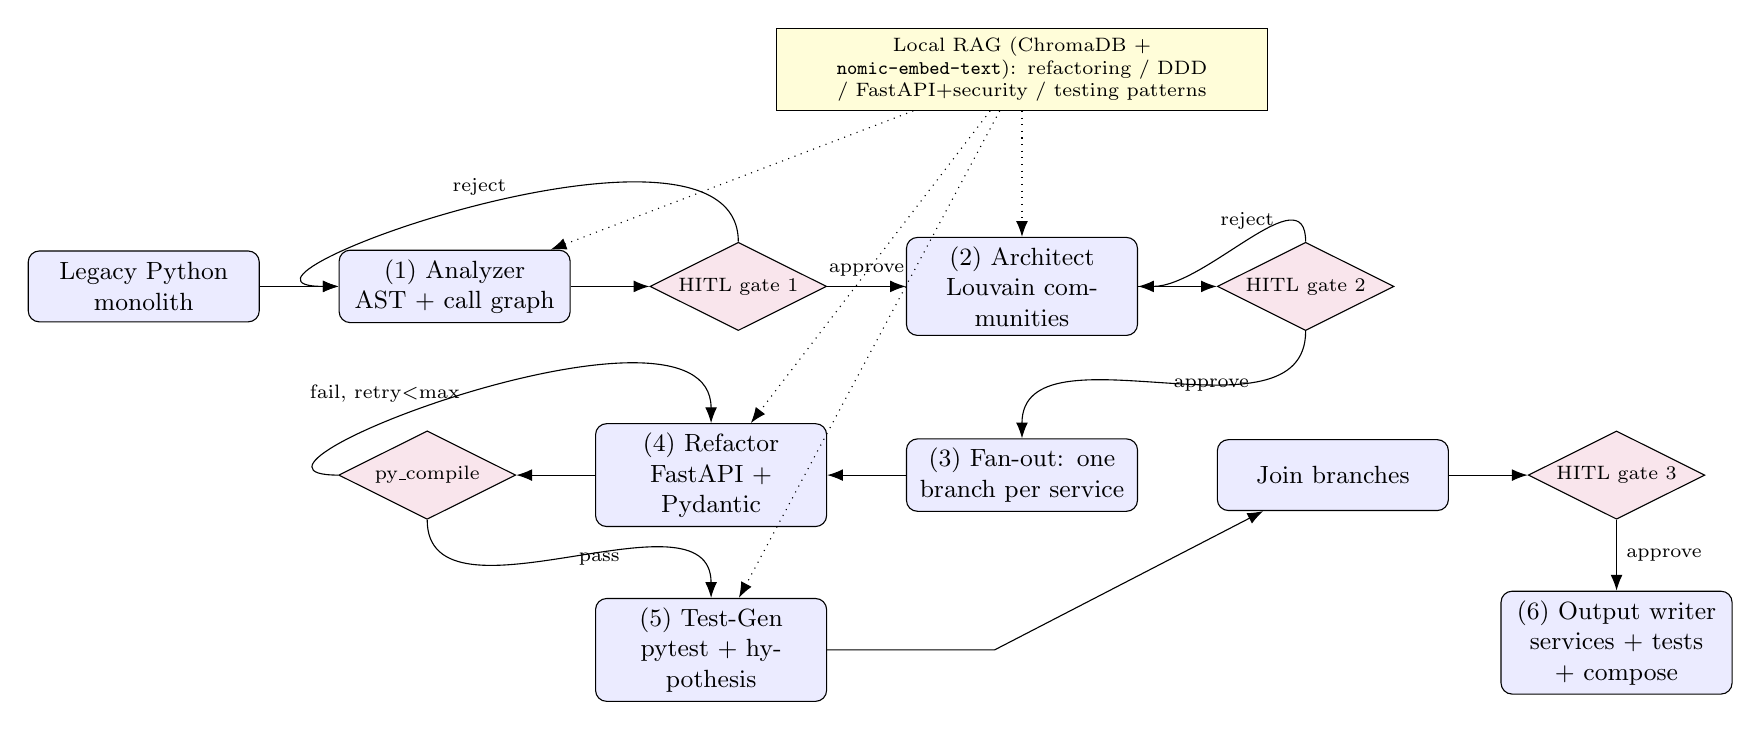
\begin{tikzpicture}[
  node distance=8mm and 10mm,
  box/.style={draw, rounded corners, fill=blue!8, align=center, minimum height=9mm, font=\small, text width=27mm},
  gate/.style={draw, diamond, fill=purple!10, align=center, font=\scriptsize, inner sep=1pt, text width=16mm, aspect=2},
  rag/.style={draw, fill=yellow!15, align=center, font=\scriptsize, text width=24mm, minimum height=8mm},
  arr/.style={-{Latex[length=2mm]}}
]
\node[box] (mono) {Legacy Python monolith};
\node[box, right=of mono] (analyze) {(1) Analyzer\\ AST + call graph};
\node[gate, right=of analyze] (gate1) {HITL gate 1};
\node[box, right=of gate1] (arch) {(2) Architect\\ Louvain communities};
\node[gate, right=of arch] (gate2) {HITL gate 2};

\node[box, below=13mm of arch, text width=27mm] (fanout) {(3) Fan-out: one branch per service};
\node[box, left=of fanout, text width=27mm] (refactor) {(4) Refactor\\ FastAPI + Pydantic};
\node[gate, left=of refactor] (compile) {py\_compile};
\node[box, below=9mm of refactor, text width=27mm] (testgen) {(5) Test-Gen\\ pytest + hypothesis};
\node[box, right=of fanout, text width=27mm] (join) {Join branches};
\node[gate, right=of join] (gate3) {HITL gate 3};
\node[box, below=9mm of gate3, text width=27mm] (output) {(6) Output writer\\ services + tests + compose};

\node[rag, above=16mm of arch, text width=60mm] (ragbox) {Local RAG (ChromaDB + \texttt{nomic-embed-text}): refactoring / DDD / FastAPI+security / testing patterns};

\draw[arr] (mono) -- (analyze);
\draw[arr] (analyze) -- (gate1);
\draw[arr] (gate1) -- node[above,font=\scriptsize]{approve} (arch);
\draw[arr] (gate1) to[out=90,in=180] node[above,font=\scriptsize]{reject} (analyze);
\draw[arr] (arch) -- (gate2);
\draw[arr] (gate2) to[out=270,in=90] node[right,font=\scriptsize]{approve} (fanout);
\draw[arr] (gate2) to[out=90,in=0] node[above,font=\scriptsize]{reject} (arch);
\draw[arr] (fanout) -- (refactor);
\draw[arr] (refactor) -- (compile);
\draw[arr] (compile) to[out=270,in=90] node[right,font=\scriptsize]{pass} (testgen);
\draw[arr] (compile) to[out=180,in=90] node[left,font=\scriptsize]{fail, retry$<$max} (refactor);
\draw[arr] (testgen) -- ++(3.6,0) -- (join);
\draw[arr] (join) -- (gate3);
\draw[arr] (gate3) -- node[right,font=\scriptsize]{approve} (output);
\draw[arr,dotted] (ragbox) -- (analyze);
\draw[arr,dotted] (ragbox) -- (arch);
\draw[arr,dotted] (ragbox) -- (refactor);
\draw[arr,dotted] (ragbox) -- (testgen);
\end{tikzpicture}%
}
\caption{End-to-end ALMS migration pipeline: deterministic structural analysis and boundary identification feed a per-service fan-out in which a local LLM agent generates code (gated by a bounded compile-retry loop) and tests, checkpointed by three human-in-the-loop gates. All LLM stages draw on a local retrieval-augmented pattern knowledge base.}
\label{fig:pipeline}
\end{figure*}

\begin{figure}[t]
\centering
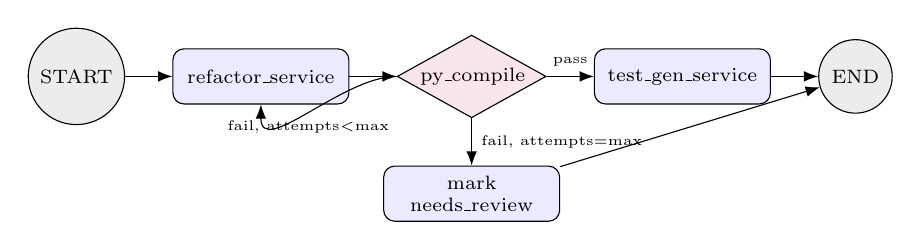
\begin{tikzpicture}[
  node distance=6mm and 6mm,
  box/.style={draw, rounded corners, fill=blue!8, align=center, minimum height=7mm, font=\scriptsize, text width=20mm},
  term/.style={draw, circle, fill=gray!15, font=\scriptsize, minimum size=6mm},
  gate/.style={draw, diamond, fill=purple!10, align=center, font=\scriptsize, inner sep=1pt, text width=13mm, aspect=1.8},
  arr/.style={-{Latex[length=1.8mm]}}
]
\node[term] (start) {START};
\node[box, right=of start] (refactor) {refactor\_service};
\node[gate, right=of refactor] (validate) {py\_compile};
\node[box, below=of validate] (review) {mark\\needs\_review};
\node[box, right=of validate] (testgen) {test\_gen\_service};
\node[term, right=of testgen] (end) {END};

\draw[arr] (start) -- (refactor);
\draw[arr] (refactor) -- (validate);
\draw[arr] (validate) to[out=180,in=270] node[below,font=\tiny]{fail, attempts$<$max} (refactor);
\draw[arr] (validate) -- node[above,font=\tiny]{pass} (testgen);
\draw[arr] (validate) -- node[right,font=\tiny]{fail, attempts=max} (review);
\draw[arr] (review) -- (end);
\draw[arr] (testgen) -- (end);
\end{tikzpicture}
\caption{LangGraph per-service subgraph (\texttt{process\_service}), run once per fan-out branch. Test generation is reached only on a compile pass and has no equivalent retry cycle of its own (Section III.F, Section V.B).}
\label{fig:orchestrator}
\end{figure}

\begin{figure}[t]
\centering
\includegraphics[width=\linewidth]{fig3_graph_comparison.pdf}
\caption{Dependency graph of \texttt{examples/sample\_monolith} before and after deterministic filtering of non-architectural calls (Python builtins, stdlib methods, local-variable methods), recomputed directly from the current Analyzer implementation. Filtering reduces the graph from 171 nodes / 267 edges / 6 hotspots to 75 nodes / 104 edges / 2 hotspots (56.1\% / 61.0\% reduction).}
\label{fig:graphfilter}
\end{figure}

\begin{table*}[t]
\centering
\caption{Comparison of monolith-to-microservice migration systems. ``Reach'' = D\textsc{ecompose} $\rightarrow$ G\textsc{enerate} $\rightarrow$ T\textsc{est} $\rightarrow$ D\textsc{eploy}.}
\label{tab:comparison}
\footnotesize
\begin{tabularx}{\textwidth}{@{}p{2.5cm}p{1.9cm}X p{1.5cm} X p{1.55cm}@{}}
\toprule
\textbf{System (year)} & \textbf{Input} & \textbf{Boundary method} & \textbf{Reach} & \textbf{LLM(s) / hardware} & \textbf{Cost / offline / HITL} \\
\midrule
Mono2Micro --- Kalia et al.\ 2021 \cite{kalia2021} & Java bytecode + traces & Hierarchical spatio-temporal clustering & Decompose only & none; local, no LLM & ---; yes; analyst review \\
MonoEmbed --- Sellami \& Saied 2025 \cite{sellami2025} & Java source (class level) & LLM embeddings + contrastive LoRA $\to$ affinity propagation & Decompose only & 18 pre-trained/benchmarked LLMs; GPU for fine-tuning & per-token API; no; none \\
Mono2Sls --- Chen et al.\ 2026 \cite{chen2026} & Python/JS source + static analysis & LLM Architect agent over static call/entry-point map & Full, to AWS SAM & Hosted: Cursor Sonnet 4.5, Claude Code Sonnet 4.6, DeepSeek-V3.2; cloud inference & \$0.58--1.06/min-app; no; 3 gates \\
Yeh et al.\ 2024 \cite{yeh2024} & Monolith tests + assumed service structure & --- (boundaries assumed) & Test only & LLM (test migration only) & ---; ---; --- \\
\textbf{ALMS (this work)} & Python monolith source & Deterministic AST call graph $\to$ builtin/stdlib filtering $\to$ Louvain (seed-fixed); LLM refines & Full, local containers & \texttt{qwen3-coder:30b} (MoE, 30.5B/3.3B active) local; \texttt{qwen2.5-coder:7b} local also validated; single CPU laptop, 16~GB RAM, no GPU & \$0; yes; 3 gates \\
\bottomrule
\end{tabularx}
\end{table*}

\end{document}
